\chapter{First Prototype Evaluation}\label{C:bin}

In chapter 4, we presented a mobile learning (m-learning) application design, the first prototype, which was developed based on Transactional Distance Theoretical-based guidelines. This chapter presents an evaluation of the prototype aiming to observe if the prototype could improve learning quality with regard to engagement and seek if there are any correlation between the engagement and learner autonomy. These findings ultimately implied the applicability of Transactional Distance Theory (TDT) to guide the design of modern education platform such as m-learning. Chapter 5 begins with explaining overall evaluation process drawing special attention to identifying participants and designing a comparative prototype. Next, we present results following by qualitative findings, their measurement methods, and technical issues happened in the actual evaluation process. Lastly, we presents how these results and findings imply the applicability of TDT to m-learning design guidelines and proposed how the prototype could be further improved. 

\section{Evaluation Process} 

There were two variables to be observed: learner autonomy and engagement. We observed learners autonomy of every participants using a pre-questionnaire (i.e., to measure motivation and confidence) and a observation of participants' actual performance of six learning tasks. This learner autonomy observation has done at the initial stage of the evaluation process. Meanwhile, for the engagement, we observed it with a post-questionnaire given after participants had finished their learning at the end of evaluation process. When participants were learning on the prototype, we video recorded their performance, tracked their interaction with Google Analytics\footnote{https://developers.google.com/analytics/solutions/mobile}, and if they initiated chat function, their conversation would be kept in a chat server located within university server, in order to observe usability and observe if participants actually interacted with the prototype. Figure 5.1 presents the laboratory setting evaluation process. 

\begin{figure}[H]
\centering
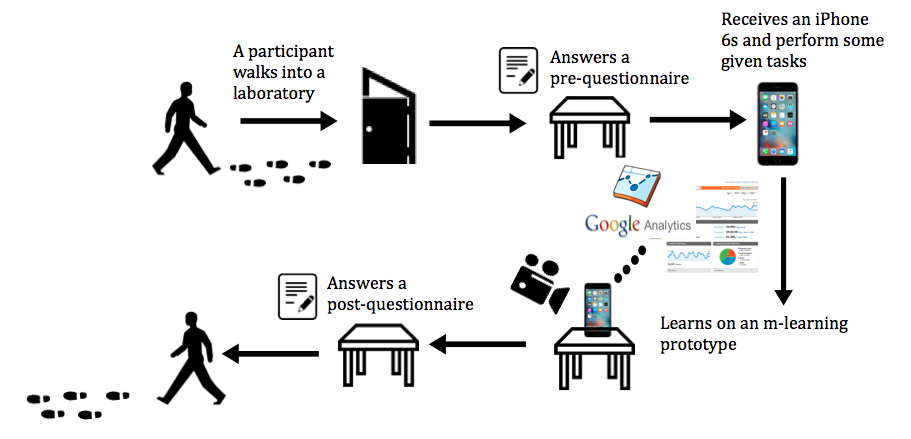
\includegraphics[width=1.0 \textwidth]{process1}
\caption{Evaluation process}
\end{figure}

\noindent\textbf{Documents}
\begin{itemize}
\item When a participant walks into a laboratory, they will receive an information sheet (Appendix B) that explained about this evaluation process and informed them that their performance would be video recorded and tracked on Goggle analytic and their chat conversation were kept on a server. 
\item They will also receive a consent form (Appendix C)
\item After that, they would receive a pre-questionnaire which used to measure motivation and confident (Appendix D) 
\item After that, we provided them an iPhone 6s and asked them to perform some tasks on the given phone and a researcher will their performance to measure knowledge and skills (Appendix E) 
\item When they finish their learning, they would receive a post-questionnaire (Appendix F)
\end{itemize} 

\textbf{Participants}
\newline
Our participants were first year engineering students at School of Engineering and Computer Science, Victoria University of Wellington. They were either enrolling for Engineering Technology (ENGR101) which introduced some fundamental technical concepts of engineering electronics, mechatronic, networked, and software systems or Introduction to Computer Program Design (COMP102) course which introduced fundamentals of programming in high-level programming language (Java). We recruited the participants by sending a classless e-mail to all the potential participants who were taking any of the courses. We used a glossary voucher to motivate them as a paid research. They were informed that any participants who actual learnt and completed the learning tasks received the voucher. We conducted the evaluation  between August \nth{10} and \nth{26} 2016, which was week \nth 5-6 of second trimester. 

From approximately 150 potential participants, 21 of them expressed their interest to participate in the study. The total of 21 participants who took part in this study, 18 were male and 3 were female. They were 17 to 22-years-old. The time the participants spent on the laboratory varied from 20 to 80 minutes. 
\newline
\newline
\textbf{A Comparative Prototype} 
\begin{itemize} 
\item \verb|P1_1| - in section 4.5, we presented an m-learning application design prototype which was developed base on Transactional Distance Theoretical guidelines. The prototype had chat function that enabled many-to-many communication between a learner, his/her teacher, and other learners, a game-based learning (i.e. quiz game), and an assignment. Additionally, it presented text, recorded audio, an animation video media. Ultimately, it had a flexible structure. That is to say, it allowed learners to access to any part of learning at any time and learn on their pace. We refer to this prototype as \verb|P1_1| 

\item \verb|P1_2| - in order to observe if the \verb|P1_1| could engage learners with their learning process, we designed another comparative prototype (\verb|P1_2|).Figures, 5.1 presents comparison of \verb|P1_1| and \verb|P1_2| prototype. The significant different between \verb|P1_1| and \verb|P1_2| were: 

\begin{enumerate} 
\item The \verb|P1_2| did not have the chat function. That is to say, learners had totally no dialogue with their teachers 
\item The \verb|P1_2| did not have recorded audio and video media. The learning content of \verb|P1_2| was presented with text media only. The is to say, there were no media used to motivate and encourage learners to learn
\item The \verb|P1_2| did not have the game-based learning function. That is to say, the application did not provided any mechanism for learners to practice what they have learnt
\item The \verb|P1_2| did not have the compulsory assignment. That is to say, learners would not receive any feedback from teachers 
\end{enumerate} 
\end{itemize}

\begin{figure}[H]
\centering
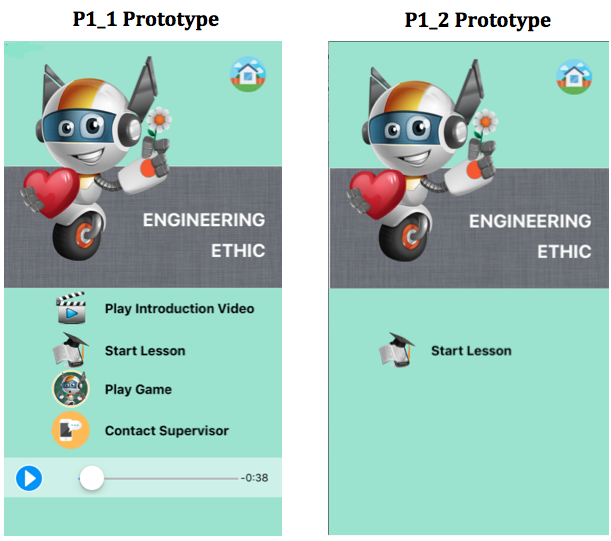
\includegraphics[width=0.6 \textwidth]{compare1}
\caption{Comparison of \detokenize{P1_1} and \detokenize{P1_2} prototype}
\end{figure}

However, to control usability variable, both prototype had the same interface design. As well as, they had the same flexibility structure. 

%%%%%%%%%%%%%%%%%%%%%%%%%%%%%%%%%%%%%%%%%%%%%

\section{Measurement and Results} 

This section presents measurement of learner autonomy and engagement as well as their correlation. 

\subsection{Learner Autonomy}
\noindent\textbf{Measurement} 
\newline
Our research investigated participants' learner autonomy using a pre-questionnaire to observe learners' motivation and confidence and using an eight tasks performance to observe learner's knowledge and skills.
\begin{itemize} 
\item The pre-questionnaire consists of three sections: students' information (i.e., gender and age), motivation section, and confident section. The motivation section consists of eleven questions and the confidence section consists of nine questions. We divided the rank of the responses from -2 to 2 (i.e., strongly disagree = -2, disagree = -1, no opinion = 0, agree = 1, and strongly agree = 2). 

\item The eight given tasks consists of connecting the given phone to an available wifi, opening a web browser, sending an e-mail, sending a text message, playing a recorded voice, playing a video, using camera to capture a photo, and creating an event on the calendar. A researcher observed how each participant performed the given tasks. We also informed every participant that the researcher could give some guidance and was willing to demonstrate how the tasks could be done if they required. 
\end{itemize}

\noindent\textbf{Results} 
\begin{itemize}
\item Results collecting from the pre-questionnaire showed that every participant had positive level of motivation and confident. Table 5.1 presents motivation and confidence level of each participants.
\newpage 
\begin{table}[H]
\centering
\setlength{\tabcolsep}{4pt}
\caption{Average level of motivation and confident of each participant}
\begin{tabular}{|c|c|c|} \hline
Participant (P) & Motivation Level & Confident Level\\
\hline
P1 & 0.64  &\cellcolor{red!25}0.33  \\
\hline 
P2 & 0.82 & 1.11   \\
\hline 
P3 & 1.82  & 1.44 \\
\hline 
P4 & 1.09 & 0.89  \\
\hline 
P5 & 1.55  & 1.00  \\
\hline 
P6 & 1.18  & 1.56  \\
\hline 
P7 & 1.27  & 1.11  \\
\hline 
P8 & 1.55  & 1.33  \\
\hline 
P9 & 0.64  & 1.00  \\
\hline 
P10 & 1.27  & 1.11  \\
\hline 
P11 & 0.82  & 0.89  \\
\hline 
P12 & 1.27  & 1.67  \\
\hline 
P13 & \cellcolor{blue!25}1.73  & \cellcolor{blue!25}1.78  \\
\hline 
P14 & 1.36  & 0.67  \\
\hline 
P15 & 0.91  & 0.67  \\
\hline 
P16 & 0.91  & 0.78  \\
\hline 
P17 & 1.18  & 1.00  \\
\hline 
P18 &\cellcolor{red!25}0.45  & 1.11  \\
\hline 
P19 & 0.82  & 0.67  \\
\hline 
P20 & 0.36  & 1.00  \\
\hline 
P21 & 1.27  &  0.67 \\
\hline 
\cellcolor[gray]{0.7}Average & \cellcolor[gray]{0.7}1.09  & \cellcolor[gray]{0.7}1.04 \\
\hline
\end{tabular}
\end{table}

\noindent The highest motivation level was 1.73 and the lowest was 0.45.
\newline \noindent The highest confident level was 1.78 and the lowest was 0.33.
\newline \noindent The average of motivation level was 1.09 and the average of confident level was 1.04.

\newpage
\item From the observation, most of the participants could perform all the eight tasks at their first attempt. None of them ask for any suggestion or demonstration from the researcher. A few of them had problem connecting the given phone to an available wifi, however they managed to complete the task within their second attempt without asking any help from the researcher. These group of participants claimed they used a different mobile operating system (i.e., Android). 
\newline
\newline \noindent Therefore, we concluded that our participants had knowledge how to perform the given tasks. Some of them had skills as they had experience using the same operating system with the given phone (i.e., Apple's iOS). Another group, who had used a different operating system, also could develop the skills on their own. 
\end{itemize}

As we mention in section 2.x, the autonomous learner was the one who had motivation, confident, knowledge, and skills all together. Based on the pre-questionnaire and the observation of the participants' performance: 
\newline 
\begin{addmargin}[1.5em]{1.5em}
\textit{\textbf{"All of the participants were autonomous learner"}}
\end{addmargin}


\subsection{Learner Engagement} 
\noindent\textbf{Measurement} 
\newline
The engagement was observe using a post-questionnaire. The questionnaire measured six concepts of engagement (i.e., focus attention, perceive usability, aesthetics, endurability, novelty, and felt involvement) used to form the questionnaire. The answers were rank from -2 to 2 (i.e., strongly disagree = -2, disagree = -1, no opinion = 0, agree = 1, and strongly agree = 2). If the questions were negative meaning, we inverted the rank. 
\newline 
\newline 
\noindent\textbf{Measurement Note} 
\newline
Even though, there were more media and learning-supported functions in \verb|P1_1| prototype, it was not compulsory that the participants who received this prototype had to use all the media and functions. Except the assignment that was compulsory, the participants made their own choice which media and functions they would like to use. Similarly, the participant who received the design \verb|P1_2| prototype also made their own choice to learn, skim, or skip any learning content. 
\newline 
\newline 
\noindent\textbf{Results} 
\begin{itemize} 
\item Average engagement level - table 5.2 and Figure 5.3 present the average engagement level of \verb|P1_1| and \verb|P1_2|. 

\begin{table}[H]
\centering
\caption{Average engagement level and standard deviation of \detokenize{P1_1} and \detokenize{P1_2}}
\begin{tabular}{|c|c|c|} \hline
 Prototype & Avg. Engagement & SD \\
\hline
\verb|P1_1|& 0.68 & 0.46 \\
\hline 
\verb|P1_2|& 0.01 & 0.59 \\
\hline
\end{tabular}
\end{table}

\begin{figure}[H]
\centering
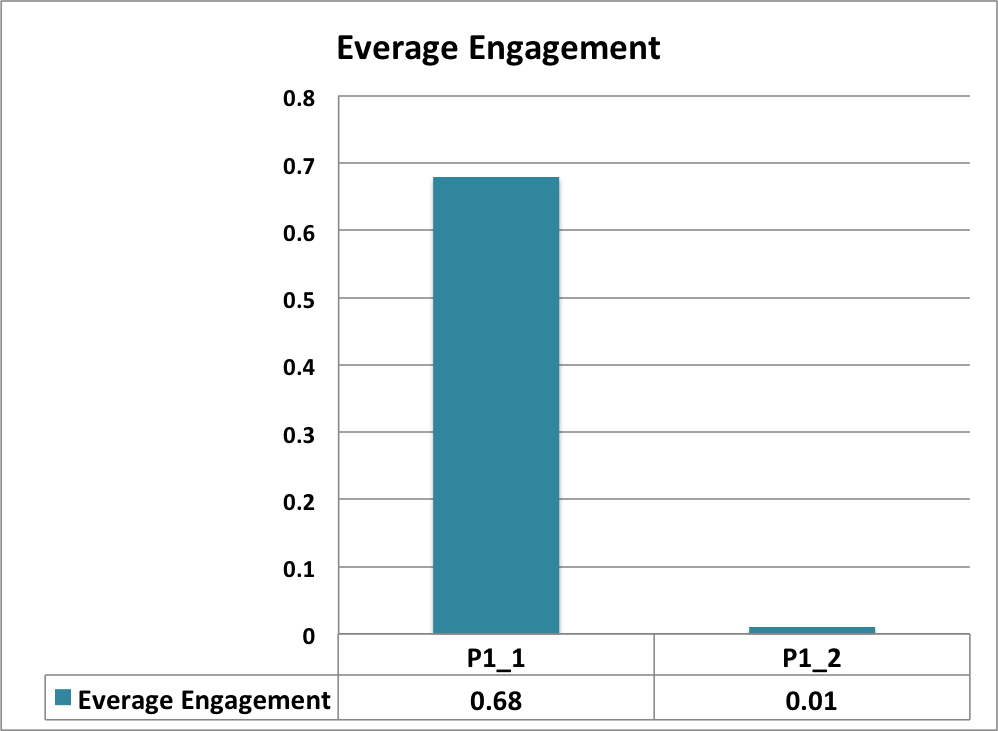
\includegraphics[width=0.6 \textwidth]{r11}
\caption{Average engagement level of \detokenize{P1_1} and \detokenize{P1_2}}
\end{figure}


Results collecting from the post-questionnaire shows that  the participants who had learnt on the design \verb|P1_1| had the average engagement level higher than the participants who learnt on the design \verb|P1_2|.

The average engagement of the \verb|P1_2| prototype got close to level zero. That is to say, overall, participants had neutral engagement toward the design. On the other hand the average engagement level of the \verb|P1_1| prototype reached to 0.68. It showed that the participants were more engaged to learning process when leant with \verb|P1_1| compared to \verb|P1_2|. 
\newline 
\begin{addmargin}[1.5em]{1.5em}
\textit{\textbf{"The m-learning application prototype that was developed base on Transaction Distance Theoretical guidelines could engage learners with their learning process"}} 
\end{addmargin}

\item Each engagement concept - table 5.3 Figure 5.4 present the average engagement level of each engagement concept of \verb|P1_1| and \verb|P1_2|. 

\begin{table}[H]
\centering
\setlength{\tabcolsep}{5pt}
\caption{Average engagement level of each engagement concept of \detokenize{P1_1} and \detokenize{P1_2}}
\begin{tabular}{|c|c|c|} \hline
Engagement Concept & \verb|P1_1| & \verb|P1_2|  \\
\hline
 \cellcolor{blue!25}Focus Attention&  \cellcolor{blue!25}0.40 (SD 0.61) &  \cellcolor{blue!25}-0.30 (SD 0.52)  \\
\hline 
\cellcolor{red!25}Usability& \cellcolor{red!25}0.84 (SD 0.52) & \cellcolor{red!25}0.64 (SD 0.79)  \\
\hline
Aesthetics & 0.64 (SD 0.99) & 0.10 (SD 1.24)  \\
\hline 
\cellcolor{green!25}Edurability & \cellcolor{green!25}0.89 (SD 0.56) & \cellcolor{green!25}0.06 (SD 0.68)  \\
\hline
Novelty & 0.60 (SD 0.61) & 0.00 (SD 0.67) \\
\hline 
Involvement & 0.70 (SD 0.41) & -0.23 (SD 0.90)  \\
\hline
\end{tabular}
\end{table}

\begin{figure}[H]
\centering
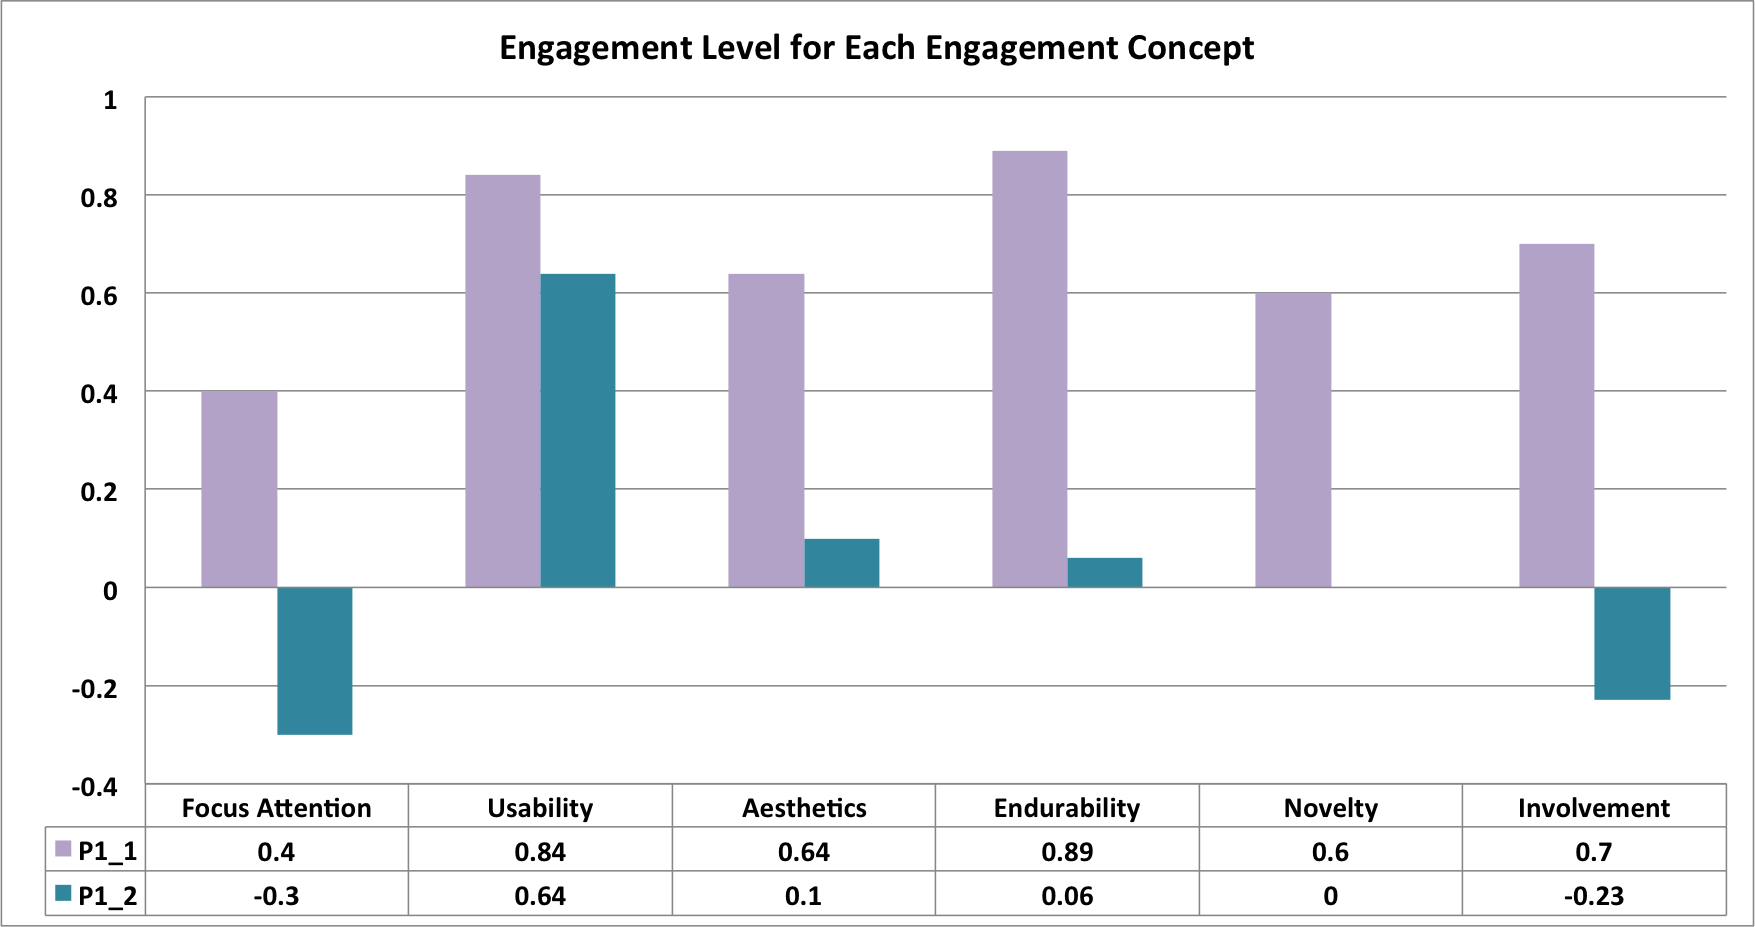
\includegraphics[width=1 \textwidth]{r12}
\caption{Average engagement level of each engagement concept of \detokenize{P1_1} and \detokenize{P1_2}}
\end{figure}

Based on the results, focus attention was the concept that the participants gave the worst response for both \verb|P1_1| and \verb|P1_2| prototypes. On the other hand, usability was the concept that the participants gave the best response for the two prototypes. 

Focus attention and involvement were the two engagement concepts that the participants who learnt on \verb|P1_2| gave a negative response. On the other hand, the participants who learnt on \verb|P1_1| gave all positive responses to every engagement concept

Edurability was the concept that had the most different value of the average engagement level between \verb|P1_1| and \verb|P1_2| design following by involvement, and focus attention. These three concepts made the most effects on the different of the overall average engagement level between the two designs

\end{itemize}




%%%%%%%%%%%%%%%%%%%%%%%%%%%%%%%%%%%%%%%%%%%%%%%%%%%%
\newpage 
\subsection{Correlation between Autonomy and Engagement}
\noindent\textbf{Measurement} 
\newline
Since the participants had been given two different types of the application design either \verb|P1_1| or \verb|P1_2| and this affected the engagement level, hence we calculate the correlation of these two group separately. 

In addition, for the autonomy, we eliminated two variables (i.e., knowledge and skills) because It was qualitative observation findings and only took motivation and confident quantitative results into calculation. The autonomy level was drawn on the average values of the motivation and confident levels. 

For a better statistical, we calculated "correlation coefficient". Our data was given in (x, y) pair (i.e., the autonomy was "x" and engagement was "y"). The correlation coefficient is: 

\begin{align*}
\hat p=\frac{S{xy}}{\sqrt{S_{xx}S_{yy}}} \ where \ &S_{xx} = \sum{x^2}- \frac{{(\sum x)}^2}n\\ 
&S_{yy} = \sum{y^2}- \frac{{(\sum y)}^2}n\\
&S_{xy} = \sum{xy}- \frac{(\sum x)(\sum y)}n\\
&and \ n \ is \ number \ of \ data \ points 
\end{align*}

We used the excel build-in function: 

= CORREL(RANE1, RANGE2) to calculate the correlation coefficient 

Statistical analysis indicated that the correlation coefficient value between -1.0 and 1.0 indicated how strongly the two variables related to each other: 
\begin{itemize}
\item The correlation coefficient is close to +1.0 indicates that there is a strong positive linear relationship between x and y (i.e., as variable x increases, variable y increases or as variable x decreases, variable y decreases).
\item The correlation coefficient is close to -1.0 indicates that there is a strong negative linear relationship between x and y (i.e., as variable x increases, variable y decrease or as variable x decreases, variable y increases).
\item The correlation coefficient is closer to 0, the less of a linear relationship between x and y exists.
\end{itemize}

\noindent\textbf{Results} 

Table 5.4 and figure 5.5 show the average autonomy and average engagement level of each participant who learnt on \verb|P1_1| and table 5.5 and figure 5.6 present the same variables of each participant who learnt on \verb|P1_2|. 

\newpage
\begin{table}[H]
\centering
\caption{Average autonomy and average engagement level of each participant who learnt on \detokenize{P1_1}}

\begin{tabular}{|c|c|c|} \hline
 Participant & Avg. Autonomy & Avg. Engagement \\
\hline
P1& 0.48 & 0.69  \\
\hline 
P3& 1.63 & 0.72 \\
\hline
P5& 1.27  & 1.66 \\
\hline 
P6& 1.37  & 0.66 \\
\hline
P9&0.82  & 0.81 \\
\hline 
P10& 1.19 & -0.05  \\
\hline
P14& 1.02  & 1.19 \\
\hline 
P15& 0.79 & 0.17 \\
\hline
P18& 0.78 & 0.43 \\
\hline 
P19& 0.74 & 0.54 \\
\hline
P21& 0.97 & 0.64 \\
\hline
\end{tabular}
\end{table}


\begin{figure}[H]
\centering
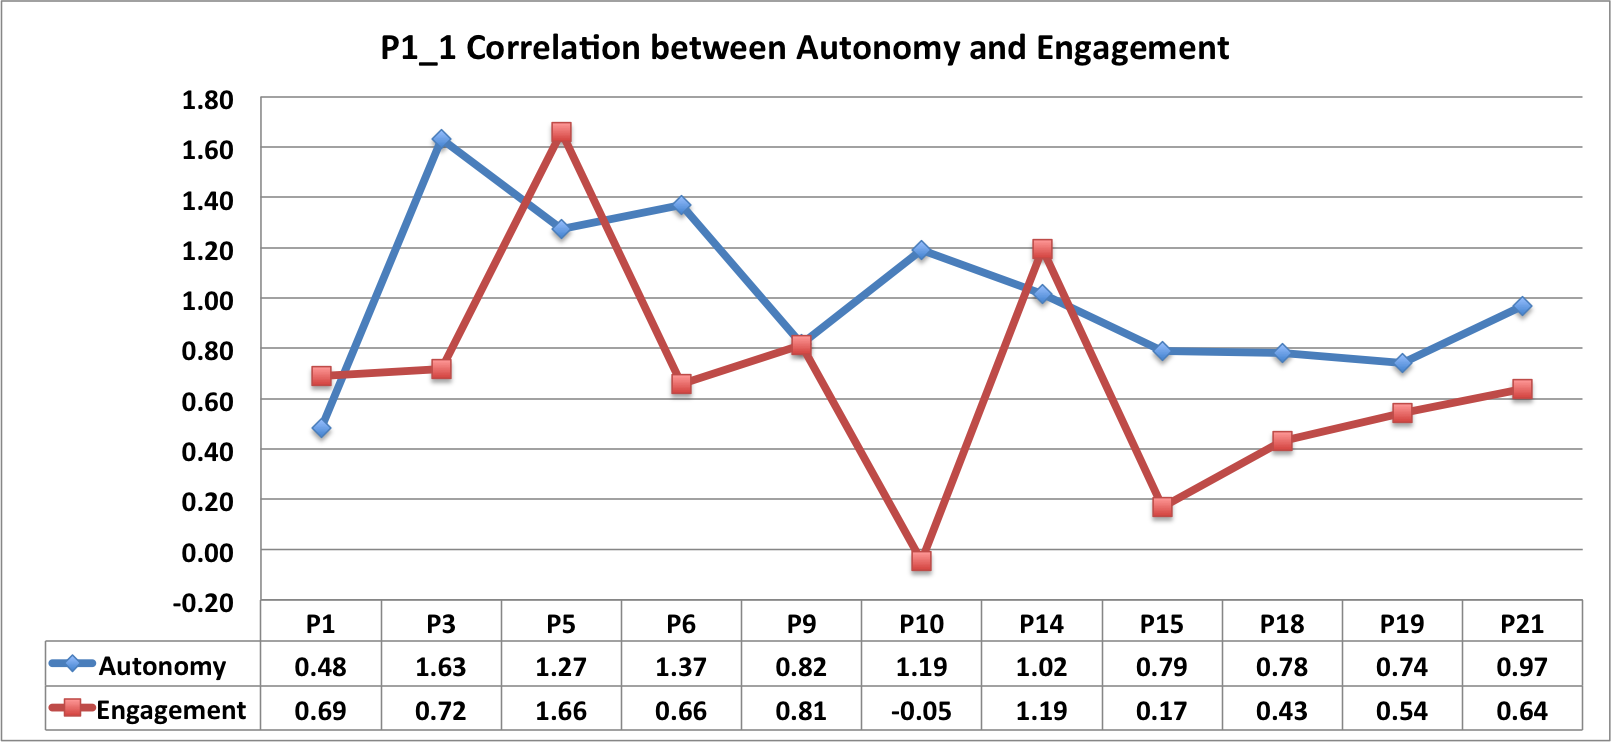
\includegraphics[width=1 \textwidth]{r13}
\caption{Illustration of the average autonomy and engagement level of the participant who learnt on  \detokenize{P1_1}}
\end{figure}
\begin{addmargin}[7em]{3em}
\textbf{The correlation coefficient of \detokenize{P1_1} was 0.21}
\end{addmargin}
\newpage 
\begin{table}[H]
\centering
\caption{Average autonomy and average engagement level of each participant who learnt on \detokenize{P1_2}}

\begin{tabular}{|c|c|c|} \hline
 Participant & Avg. Autonomy & Avg. Engagement \\
\hline
P2& 0.96  &0.23  \\
\hline 
P4& 0.99 & -0.41 \\
\hline
P7& 1.19  & 0.28 \\
\hline 
P8& 1.44  & 0.32  \\
\hline
P11&0.85  & -0.61 \\
\hline 
P12& 1.47 & 0.39  \\
\hline
P13& 1.75  & -0.79 \\
\hline 
P16& 0.84 & 0.72 \\
\hline
P17& 1.09 & -0.74 \\
\hline 
P20& 0.68 & 0.72 \\
\hline
\end{tabular}
\end{table}


\begin{figure}[H]
\centering
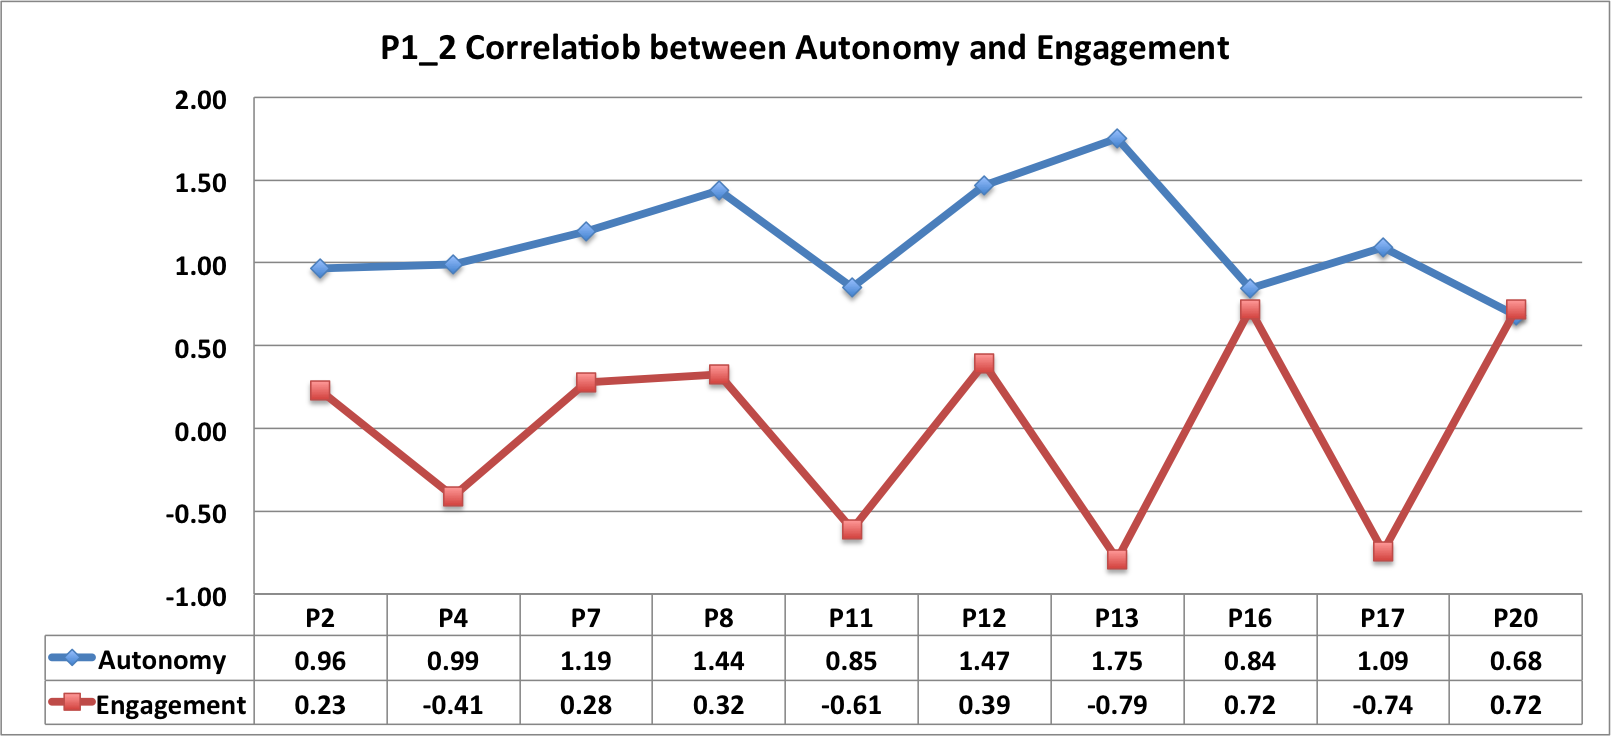
\includegraphics[width=1 \textwidth]{r14}
\caption{Illustration of the average autonomy and engagement level of the participant who learnt on  \detokenize{P1_2}}
\end{figure}
\begin{addmargin}[6.5em]{3em}
\textbf{The correlation coefficient of \detokenize{P1_2} design was -0.31}
\end{addmargin}
\newpage 
Based on the results, the correlation coefficients of both designs were close but not equal to 0. Therefore, the average autonomy and engagement of both designs were slightly correlated.
\begin{itemize} 

\item For \verb|P1_1| design, the correlation coefficient came out in a positive value. Hence there was a positive linear relationship between the two variables. In the other word, the better the participants could learn autonomously, the more they engaged with the design. 


\item For the \verb|P1_2| design, the correlation coefficient came out in a negative value. Hence there was a negative linear relationship between the average autonomy and engagement level. To put it another way, the better the participants could learn autonomously, the less they engaged with the design. 

\end{itemize}


%%%%%%%%%%%%%%%%%%%%%%%%%%%%%%%%%%%%%%%%%%%%%%%%%%%%



\section{Interface Design Observation Findings} 

The participants had been informed that their action on the screen has been video capturing, they were being tracked on the Google analytics, and had been and notified that any conversation they made on the chat room would be kept on the server. We allowed every participant to ask any questions about the evaluation before the process had begun. All the participants had given their consent to participate in this evaluation. 
\newline 
\newline 
\noindent\textbf{Observation Note} 
\newline
The pop-up, sided-slid, and drop-down menu interface design and media text existed in both \verb|P1_1| and \verb|P1_2| therefore the results were obtained from all 21 participants. Meanwhile, other learning-supported functions (i.e., the animation video, recorded audio, chat, quiz game and assignment) existed only in the \verb|P1_1|, therefore the results were obtained from only 11 participants who were assigned to learn on this prototype. 
\newline 
\newline
\noindent\textbf{Pop-up Menu} 

\begin{itemize} 
\item From the total of 21 participants, 18 of them successfully used this menu interface design and learnt on the information given the pop-up windows. Among them, only less than half (7 participants) could find the provided button right away. However, the rest of them tapped on the labels (not the pop-up buttons) several times (See figure 5.7) before they found the right pop-up buttons. These participants either found the right pop-up buttons by listening to the recorded-audio that guided "Please tab on each icon to reveal further explanation" or figured it out by themselves. 

\begin{figure}[H]
\centering
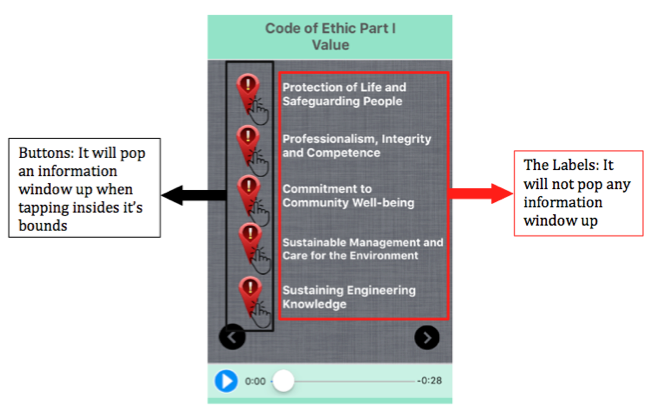
\includegraphics[width=1 \textwidth]{p1ql1}
\caption{Pop-up buttons and labels' bounds}
\end{figure}

\item 3 of them visited this learning screen but unsuccessfully popped up the information windows on the screen. Despite, listening to the guidelines given in the recorded-audio, s/he still could not perform the pop-up window. The rest of them tapped to the wrong places several times, skipped this screen, and missed all the learning content on the screen. 

\end{itemize} 

 

%%%%%%%%%%%%%%%%%%%%%%%%%%%%%%%%%%%%%%%%%%%%%%%%%%%%%%%%%%%%%%%%%%%%%%%%%%%%%

\noindent\textbf{Sided-slide Menu} - the learning content we put in the sided-slide menu interface were presented in a textbox interface that allowed the participants to copy, highlight, and scroll up and down to see the whole text.

\begin{itemize} 

\item All the 21 participants visited this screen and could find the "more item'' button which revealed the sided menu and tapped on the menu and learnt on the learning content hidden in the menu. Among them, 11 participants successfully found the buttons, tapped on it, and saw the sided-slide menu at their first attempt. The rest of them could not find the button at their first attempt. They had some confusing fingers either tapping on some wrong places or going back and forth between this screen and the other screens for several times before managed to find the button and tapped on it. 

\item All of them, scrolled up and down to read the entire learning content given in the textbox, however non of them tried to copy or highlight the text. 

\end{itemize} 


%%%%%%%%%%%%%%%%%%%%%%%%%%%%%%%%%%%%%%%%%%%%%%%%%%%%%

\noindent\textbf{Dropped-down Menu}- same with the sided-slide menu, the learning content we put in the sided-slide menu were presented in a textbox interface that allowed the participants to copy, highlight, and scroll up and down to see the whole text.

\begin{itemize}
\item From 21 participants, 20 of them visited this screen and could find the "more item" button which revealed the dropped-down menu and tapped on the menu and learnt on the learning content hidden in the menu. Among them 15 participants successfully found the buttons, tapped on it, and saw the sided-slide menu at their first attempt. The rest of them could not find the button at their first attempt. They had some confusing fingers either tapping on some wrong places or going back and forth between this screen and the other screens for several times before managed to find the button and tapped on it. 
\item 1 participant did not visit this learning screen 
\item Same with the sided-slide menu, all of them, scrolled up and down to read the entire learning content given in the textbox, however non of them tried to copy or highlight the text. 
\end{itemize}

%%%%%%%%%%%%%%%%%%%%%%%%%%%%%%%%%%%%%%%%%%%%%%%%%%%


\section{Media Observation Findings} 
\noindent\textbf{Media Text} 
\begin{itemize}
\item The media text was put in either the information window in the pop-up menu or in text boxes. The size of the provided text was equal throughout the application. We found that, none of the participants made zoom gesture neither copy or highlight the text. They seemed to have no problem reading the provided text as it was and without any prior guide, all of them could scroll up and down to see the whole text. 

\item Most of the participants learnt all the provided learning content. Even through, we could see some skim-reading as they did not spent adequate time on the screen and some text content were skipped. All of them had learnt some thing by reading the provided text content. 
\end{itemize} 

%%%%%%%%%%%%%%%%%%%%%%%%%%%%%%%%%%%%%%%%%%%%%%%%%%%%

\noindent\textbf{Media Animation Video} - the animation video introduced the learning topic (i.e., engineering ethics) and explained the learning content briefly. The main purpose of the media was to engage and motivate learners at the beginning of the learning lesson. Hence, we expected the participants to watch the video before they started to learn. 

\begin{itemize}
\item From the total 11 participants, all of them visited the video screen before they started to learn, however only 5 of them watched the video from the beginning to the end. Among them, only 1 participant watched the video one than one time. This participant also the only one who used fast forward button. 
\item Despite visiting the video screen and listening to the recorded-audio that explained the video, 6 participants leaved the video screen without playing the video. 
\end{itemize}


%%%%%%%%%%%%%%%%%%%%%%%%%%%%%%%%%%%%%%%%%%%%%%%%%%

\noindent\textbf{Media Recorded-audio} - there were seven recorded-audio files in the prototype. 

\begin{itemize}
\item Most of the participants chose to listen to the recorded-audio before start learning by reading the provided text. 
\item From the total of 11 participants, all of them listened to at less one of the recorded voice provided in the application. Among them, 6 participants listened every recorded-audio from the beginning to the rest of them only listened to some of the recorded-audio. 
\end{itemize}


%%%%%%%%%%%%%%%%%%%%%%%%%%%%%%%%%%%%%%%%%%%%%%%%%%%%%%%

\section{Learning Supported Functions Observation Findings}

\textbf{Function Chat} - the chat function was designed as a communication channel between participants and their instructor. The participants were informed that they could ask any question through the chat room. A researcher took a role-play as the instructor. This function was not a compulsory function that the participants needed to use. It was their choice if they wanted to initiated conversation. 

One key thing to note was the design of the chat function had a problems. The chat room could not be exited therefore any participants who used the chat must reset the application to exit the chat and start the application again to continue their learning process. These might affect the participants' engagement. 

\begin{itemize}
\item From the total of 11 participants, 8 of them used the chat function. Figure 5.8 shows some examples of the chat conversation between the participants and the instructor. 

\begin{figure}[!hbt]
\centering
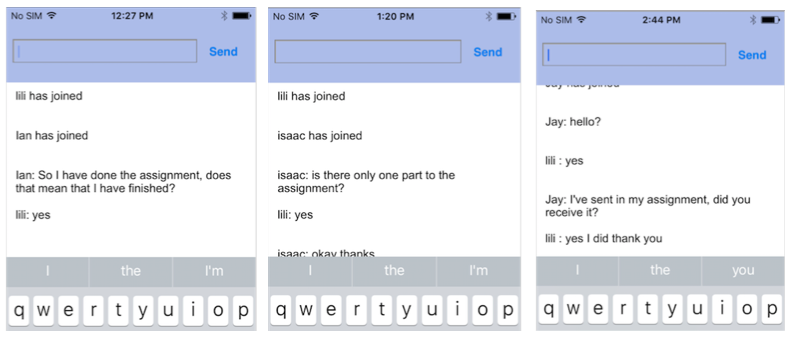
\includegraphics[width=1 \textwidth]{p1ql5}
\caption{Chat conversation between the participants and the researcher}
\end{figure}

Among them, 3 participants used the chat to ask about the given assignment. The chat conversation were: 

\verb|``... Participant_1: hi|\hfill
	\newline \verb|Participant_1: I have a question|\hfill 
       	\newline \verb|Instructor: Hi, please ask|\hfill
       \newline \verb|Participant_1: do I need to answer the question now?|\hfill
       \newline \verb|Instructor: Yes, you can click on the answer button|\hfill
       \newline \verb|and answer a short one.|\hfill
       \newline \verb|Participant_1: what do I have to describe about?|\hfill  
       \newline \verb|Instructor: Do you think Facebook should treat|\hfill 
       \newline \verb|teenager differently ...''|\hfill
\newline\newline \verb|``... Participant_2: is there only one part of the|\hfill
\newline\verb|assignment?|\hfill
      \newline\verb|Instructor:	yes|\hfill 
      \newline\verb|Participant_2: 	okay thanks ...''|\hfill 
\newline\newline \verb|``... Participant_3: hi|\hfill 
      \newline\verb|Participant_3: does the assignment want me to talk|\hfill
      \newline\verb|about the different in treating teenagers differently?|\hfill
       \newline \verb|Instructor: No, you need to answer if you think|\hfill
       \newline \verb|they should be treated differently and why.|\hfill
       \newline\verb|Answer a short one.|\hfill
       \newline\verb|Participant_3: okay thanks ...''|
\newline 
\newline \noindent and 3 participants asked if they had performed correctly and ensure if their assignment was received. The chat conversation were: 

\verb|``... Participant_4: I've sent in my assignment,|\hfill
\newline\verb|did you receive it?|\hfill
      	      \newline \verb|Instructor: yes I did thank you|\hfill 
      	      \newline \verb|Participant_4: awesome ...''|\hfill
\newline \newline \verb|``... Participant_5: Is there only one question?|\hfill
      	      \newline \verb|Instructor: yes ...''|\hfill 
\newline \newline \verb|``...Participant_6:	So I have done the assignment,|\hfill
\newline\verb|does that mean I have finished?|\hfill 
      	  \newline \verb|Instructor: yes ...''|
\newline 
\newline \noindent The other 2 participants used the chat to inform that they have done their learning. 

\item 3 participants who did not use the chat function to contact the supervisor. We have checked their learning process; two of them seemed to learn smoothly and had no problem to find the buttons and learning screens on their own. Meanwhile, 1 participant seemed to have problem navigating through the learning content, however at the end s/he managed to find the way by him/herself. 
\end{itemize}

%%%%%%%%%%%%%%%%%%%%%%%%%%%%%%%%%%%%%%%%%%%%%%%%%%%%%%%%%%%%%%%%%

\noindent\textbf{Quiz Game} - same as the chat function, it was not compulsory to play the quiz game. It's the participants' choice if they wanted to practice and challenge themselves. 
Form the total of 11 participants, 10 of them played game at less after they had learnt the given text content. Among them, 5 participants played game once, 3 participants played game more than one time. 

%%%%%%%%%%%%%%%%%%%%%%%%%%%%%%%%%%%%%%%%%%%%%%%%%%%%%%5


\noindent \textbf{Assignment} - the assignment was the only compulsory function in the \verb|P1_1|. The participants were informed that they had to finish the assignment and sent it to the instructor via a given e-mail platform. The assignment was a reading case study and the participants had to express their opinion in a short answers 5-7 sentences. 

\begin{itemize}
\item From the total of 11 participants, all of them successfully submitted their assignment and we received it through the e-mail. 
\item All the answer we received had proved that the participants understood the case study. Figure 5.9 shows two of the answer in the e-mail platform we received from the participants. 
\item Another purpose of asking the participants to type in the short answer was to observe if the small keyboard of the iPhone 6s bother them. We found that it did not seem to cause frustration. All of the participants typed in the answer using either only one or many fingers pretty fast. They seemed to have no problem with the small keyboard and they rarely made a mistake typing on the keyboard. 
\end{itemize}
\newpage 
\begin{figure}[H]\centering
    \begin{subfigure}{0.8\textwidth}
 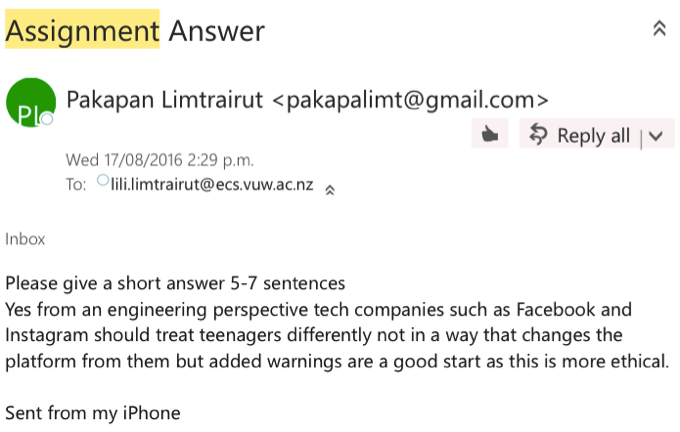
\includegraphics[width=\textwidth]{p1ql6a}
 \caption{Assignment example 1}
    \end{subfigure}\hspace{0.1\textwidth}
    \begin{subfigure}{0.8\textwidth}
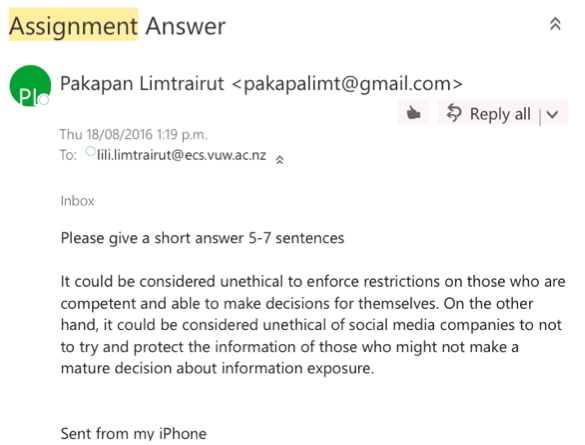
\includegraphics[width=\textwidth]{p1ql6b}
  \caption{Assignment example 2}
    \end{subfigure}
    \caption{Assignment answers sent from the participants to the researcher's email}
\end{figure}


%%%%%%%%%%%%%%%%%%%%%%%%%%%%%%%%%%%%%%%%%%%%%%%%%%
\section{Observation Issues}

The camera was set statically and there were some moments when the participants lifted their arm up and switched between left and right hand. They unintended blocked the mobile phone's screen, or the mobile phone's screen was out of the video recording frame. Figure 5.10 shows the moments when we could not see the phone's screen clearly. 

\begin{figure}[!hbt]
\centering
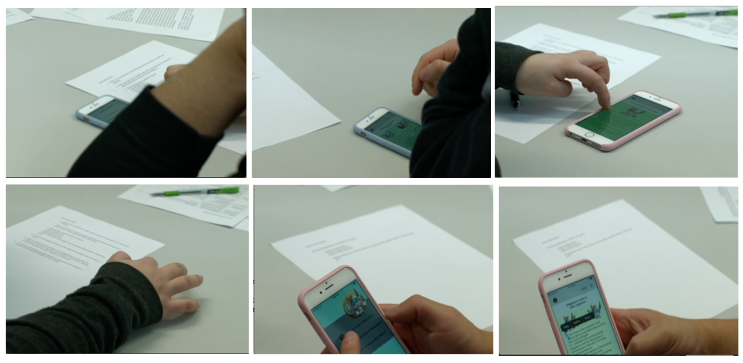
\includegraphics[width=1 \textwidth]{issue}
\caption{The screen capture of the moments when the mobile phone's screen were blocked or out the frame}
\end{figure}

Fortunately, the moments were brief and did not affect much on the observation results. Any moment seemed to be significant important to the observation. We double-checked the results from Google analytics website. The number of the tabbing on the buttons reported on the Google analytics should conform to what we saw from the video. If the number were not the same, we followed the report from Google analytics and concluded that the participants had performed the tabbing when we could not see the screen. 

%%%%%%%%%%%%%%%%%%%%%%%%%%%%%%%%%%%%%%%%%%%%%%%%%%%%%%%%
\newpage
\section{Analysis} 

\begin{itemize} 
\item Pop-up menu interface design - Base on the results, the pop-up design had potentials to present learning content to learners. However, there was some design awareness: 
\begin{itemize}
\item As the nature of pop-up design, the learning content will be hidden inside a button, if the button is not tapped on the learning content will not be reveal and learners will miss the entire learning content.
\item The pop-up buttons should be effortlessly visualized. The image or label that are located in the same screen with the buttons but does not pop any information window ups, could lead to frustration and confusion. 
\item There should be a guide (e.g., a recoded voice, a guided text, or a pointer) to inform learners to tab on the right pop-up button. 
\end{itemize}

\item Sided-slide menu interface design - Based on the results, the sided-slide menu interface design had more potential to present learning content compare to the pop-up interface style. Despite, many participants struggled to find the button that revealed the menu in the first time. 

The only suggestions for this interface design were making the ``more info'' button to be more attractive and stand out from the background. In addition, a guide (e.g., a recoded voice, a guided text, or a pointer) can be used to inform learners to tab on the button and the provided menu.

\item Dropped-down menu interface design - Based on the results, the drop-down menu interface design also had potential to present learning content. However, we strongly believed that the higher percentage of the successful finding the menu at the first attempt of the drop-down menu was influenced by the fact that they had learnt the location of the menu from the previous learning section. Therefore, we would suggest making the ``more info'' button to be more attractive and stand out from the background. In addition, a guide (e.g., a recoded voice, a guided text, or a pointer) can be used to inform learners to tab on the button and the provided menu. Note that, all the participants had experienced interacting with the sided-slide before they saw the drop-down menu interface design and the ``more info'' buttons of the two interface designs were located at the same place (i.e., the top-right corner of the screen). Therefore the participants might know where they should look for the button. This may influence the results and raise the percentage of the successful finding the menu at the first attempt. 

\item Media text - We found no design awareness towards this type of media. It could bring the learning content across to the participants. 
\item Animation Video - The reason for this interaction might came from the wrong guidance we provided in the voice file that said : 
`` …................ for more detail please start the lessons''

The participants then went out from the video screen to start the lessons without tabbing on the ``play video''. Based on the observation results, video media was a powerful media that had potential to catch participants' interests at the beginning of the lesson as all of them visited the video screen before started their lessons. However, there was some design awareness: 
\begin{itemize}
\item The ``play video'' button should be appealing, stands out from the background, and locate at the obvious spot.
\item The recorded voice was actually a good accompanied media of the video. As many participants listened to it before started to watch the video. However, the recoded voice should guide learners to watch the video by tabbing on the provided ``play button''. The misguided recorded voice could lead to confusion. The video might not be played and cause a lost of a chance to attract and engage learners. 
\end{itemize}

\item Based on the observations, the recorded voice seemed to be a powerful media bringing the learning content across to the participants especially to introduce learning topic to learners. 

The recorded voice leaded to a misunderstanding and many participants did not watch the video. Therefore, if the recorded voice is used to guide learners, make sure that the guidance is accurate. 

\item Based on the observations, the chat was useful for the participants when they had a question and they would like to confirm if their had done the given correctly. 

\item Based on the findings, game was well accepted by the participants. Around 90\% of them chose to play game after they had done their learning. We did not find any design issue against the game design. Every participant could navigate through the game from the beginning to the end smoothly. 

\item Based on the findings, most of participants who used the chat function, asked about the assignment. Therefore, it was a good function that could enhance the communication between the participants and the instructors. The case study type of question was an acceptable type of question. Similarly, the short answer that requires the participants to type in also an acceptable type of answer on the m-learning application. 

\end{itemize} 
%%%%%%%%%%%%%%%%%%%%%%%%%%%%%%%%%%%%%%%%%%%%%%%%%%%%%%%%

\section{Summary}

In this chapter, we presented the results, findings, and data analysis of data we obtained from the first evaluation iteration. The main goals of the evaluation were to observe the actual performance of the first prototype design (P1) and to compare the learning effectiveness in regarding to engagement of the design that followed TDT design guidelines (\verb|P1_2|) and the design that did not follow the guidelines (\verb|P1_1|). 

In order to achieve the first goal, we invited the target learners to try the P1 in a laboratory setting. We video recorded on the mobile phone screen and transcribed the video as well as tracked their interaction with Google analytics. Then we transcribed the video and summarize if the participants had an actual learning, how much they had learnt and if there were any interface design problems that might cause the failure. For the second goal, we divided the participants into two groups and asked them to perform either \verb|P1_1| or \verb|P1_2| design. We used a post-questionnaire to evaluate the engagement level. 

Research outcomes we presented in this chapter were the interface design guidelines and design awareness, the qualitative explanation how the provide media (i.e., text video, and recorded voice) had been used, statistical analysis of the average engagement level of \verb|P1_1| and \verb|P1_2| design, statistical analysis of average learner autonomy of the participants, and the statistical analysis of the correlations between the average autonomy and engagement level. 

Firstly, the interface pop-up, sided-slide, and dropped-down menu designs successfully presented learning contents to the participants. Majority could find the menus at their first attempt, minority took some times to figure out how to use the design, and less could not use the provided menus. Significantly, every participants got to learn either the entire learning content provided in the application or at less a part of it. Having said that, the ``menu button'' within the interface design should be appealing and stand out from the background. What's more, the button should be accompanied with a guidance or pointer. A recorded voice, a pointing arrow, or a text explanation, for instance, can lead the participants to click on the right button. 

Secondly, the participants actual learnt by reading the provided media. They read the provided text within textbox interface design. Even though, we provided a zoom-in zoom-out, copy, and highlight functions for the text, none of the participants had used them. The recorded voice was the media that most participants used before they started their learning. Hence, it is suitable media for an introduction or guiding at the beginning of the learning lesson. Video was the other media we put the prototype design with an aim to attract the participants at beginning of learning lesson. However, we provided a misguided recorded voice and the ``play button'' wasn't visual appealing, half of the participants did not get to watch the video. 

Thirdly, \verb|P1_2| could engage the participants better than \verb|P1_1|, provided that the \verb|P1_2| had a design problem (i.e., the chat function could not be exited and the application needed a reset). Another key thing to remember is the provided media and functions we provided in \verb|P1_2| design were not compulsory for the participant to use. That is to say, we provided the media and functions based on TDT guidelines however it was the participants’ choice if they wanted to use them. 

Fourthly, the participants were autonomous learners. In other words, they had knowledge, skill, motivation and confidence to learn on a smart phone. 

Lastly, the average autonomy and engagement level were slightly correlated. However, the correlation for the \verb|P1_1| and \verb|P1_2| design were inverse trend. For the \verb|P1_1| design, the better the participants could learn autonomously the less they engaged to the design. For the \verb|P1_2| design, the better the participants could learn autonomously, the more they engaged with the design. 

%%%%%%%%%%%%%%%%%%%%%%%%%%%%%%%%%%%%%%%%%%%%%%%%%%%%%%%%%%%


